\documentclass[10pt]{beamer}
\usetheme{jambro}

\title[]{Macroeconomia I - Curva de Phillips, taxa natural de desemprego e inflação}
\author[]{\href{https://pvfonseca.github.io}{Paulo Victor da Fonseca}}
\date{}

\hypersetup{
    colorlinks = true,
    urlcolor = teal,
    linkcolor = teal    
}
\usepackage[portuguese]{babel}
\usepackage{subfig}
\usepackage{emoji}
\usepackage{hyperref}

\begin{document}

\begin{frame}[plain]
    \titlepage{
        \begin{center}
            \begin{minipage}{0.8\textwidth}
                \centering
            \end{minipage}
        \end{center}}
\end{frame}

\begin{frame}{Sumário}
    \tableofcontents
\end{frame}

\section{Introdução}
\begin{frame}{Introdução}
    \begin{itemize}
        \item Em 1958, A. W. Phillips, um economista neozelandês e, então, professor da London School of Economics, publicou um estudo abrangente do comportamento dos salários no UK para os anos de 1861 a 1957.
        \bigskip
        \begin{figure}
            \centering
            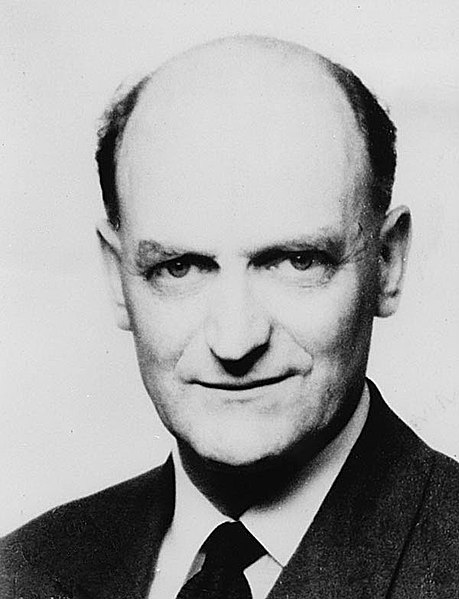
\includegraphics[width=0.2\textwidth]{./figures/aula13_fig1.jpg}
            \caption{Alban William Housego Phillips (1914-1975). Fonte: \href{https://en.wikipedia.org/wiki/William_Phillips_(economist)}{Wikipedia}.}
            \label{fig1}
        \end{figure}
    \end{itemize}
\end{frame}

\begin{frame}{Introdução}
    \begin{itemize}
        \item A principal descoberta está resumida na Figura \ref{fig2}, reproduzida a partir de seu artigo.
    \end{itemize}
    \begin{figure}
        \centering
        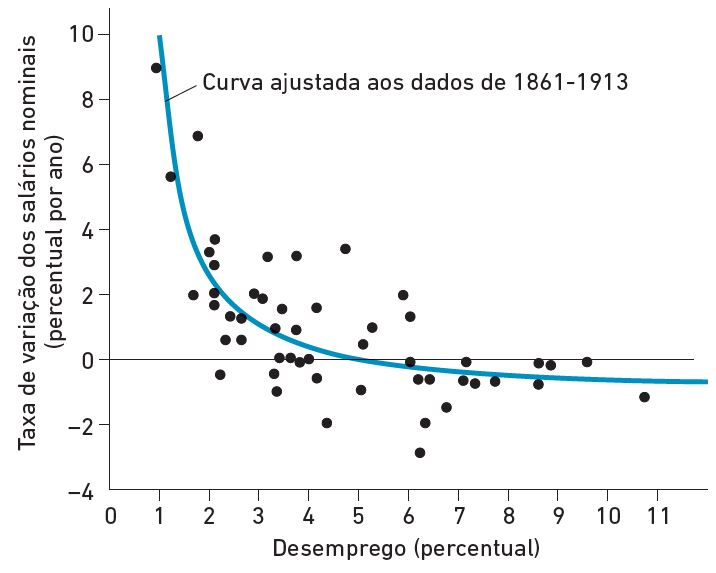
\includegraphics[width=0.5\textwidth]{./figures/aula13_fig2.JPG}
        \caption{A curva de Phillips original para o Reino Unido. Fonte: Dornbusch et al. (2013).}
        \label{fig2}
    \end{figure}
\end{frame}

\begin{frame}{Introdução}
    \begin{itemize}
        \item Phillips encontrou claras evidências de uma relação negativa entre inflação e desemprego.
        \bigskip
        \item Quando o desemprego era baixo, a inflação era alta.
        \bigskip
        \item Quando o desemprego estava alto, a inflação estava baixa - até mesmo negativa (deflação).
        \bigskip
        \item Essa relação empírica negativa entre desemprego e inflação (ou taxa de aumento dos salários nominais) ficou conhecida como \textcolor{blue}{curva de Phillips}.
    \end{itemize}
\end{frame}

\begin{frame}{Introdução}
    \begin{itemize}
        \item Dois anos depois, Paul Samuelson e Robert Solow repetiram o exercício para os Estados Unidos, com dados de 1900 a 1960.
    \end{itemize}
    \begin{figure}
  \centering
  \subfloat[Paul Samuelson (1915-2009)\label{fig3a}]{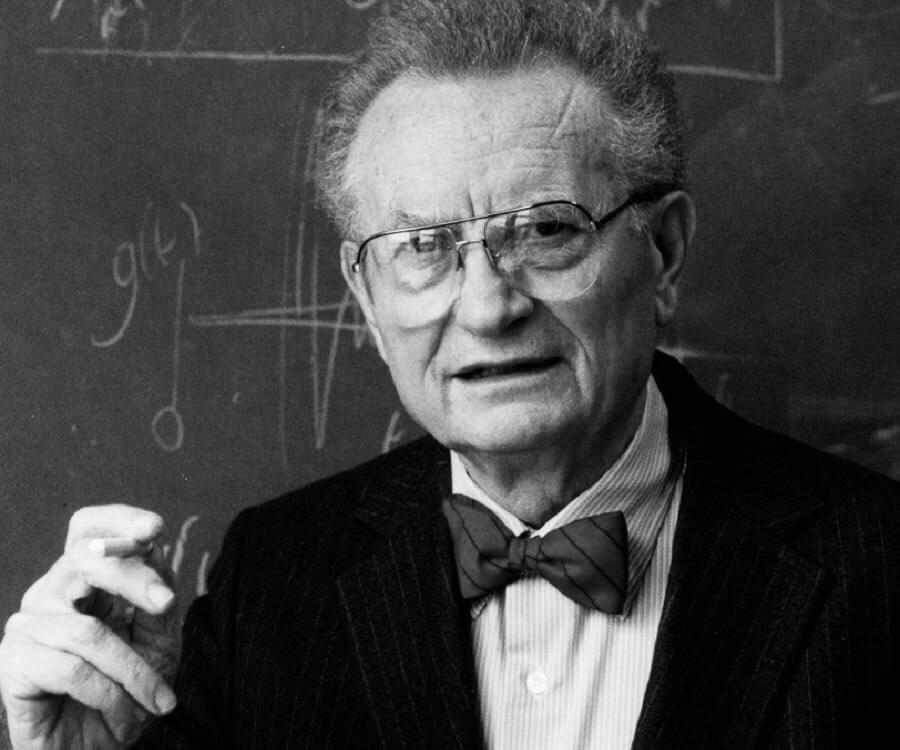
\includegraphics[width=0.4\textwidth]{./figures/aula13_fig3.png}}\qquad
  \subfloat[Robert Solow (1924 - )\label{fig3b}]{
\includegraphics[width=0.4\textwidth]{./figures/aula13_fig4.jpg}}
\caption{Paul Samuelson e Robert Solow - Prêmio Nobel de Economia em 1970 e 1987, respectivamente.}
\label{fig3}
\end{figure}
\end{frame}

\begin{frame}{Introdução}
    \begin{itemize}
        \item A Figura \ref{fig4} reproduz suas conclusões usando a inflação do índice de preços ao consumidor dos EUA como medida da taxa de inflação.
    \end{itemize}
    \begin{figure}
        \centering
        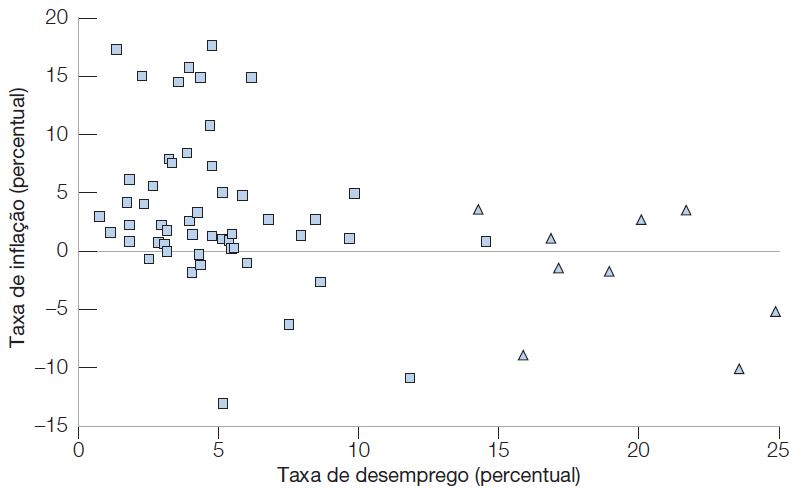
\includegraphics[width=0.6\textwidth]{./figures/aula13_fig5.JPG}
        \caption{Inflação $\times$ desemprego nos EUA, 1900-1960. Fonte: Blanchard (2017).}
        \label{fig4}
    \end{figure}
\end{frame}

\begin{frame}{Introdução}
    \begin{itemize}
        \item Exceto pelo período de acentuado desemprego na década de 1930 (representados por triângulo na Figura \ref{fig4}), também parece haver uma clara relação negativa entre inflação e desemprego nos EUA.
        \bigskip
        \item A relação negativa entre desemprego e inflação da curva de Phillips - termo cunhado por Samuelson e Solow - tornou-se fundamental tanto para o pensamento quanto para políticas macroeconômicas.
        \bigskip
        \item Ela parecia implicar que os países poderiam escolher entre combinações diferentes de desemprego e inflação (\textcolor{blue}{trade-off desemprego $\times$ inflação}).
        \bigskip
        \item Muito da discussão sobre política macroeconômica tornou-se, então, uma questão acerca de qual ponto escolher na curva de Phillips.
    \end{itemize}
\end{frame}

\begin{frame}{Introdução}
    \begin{itemize}
        \item Um exemplo significativo da curva de Phillips ocorreu nos Estados Unidos durante a década de 1960, conforme visto na Figura \ref{fig5}.
    \end{itemize}
    \begin{figure}
        \centering
        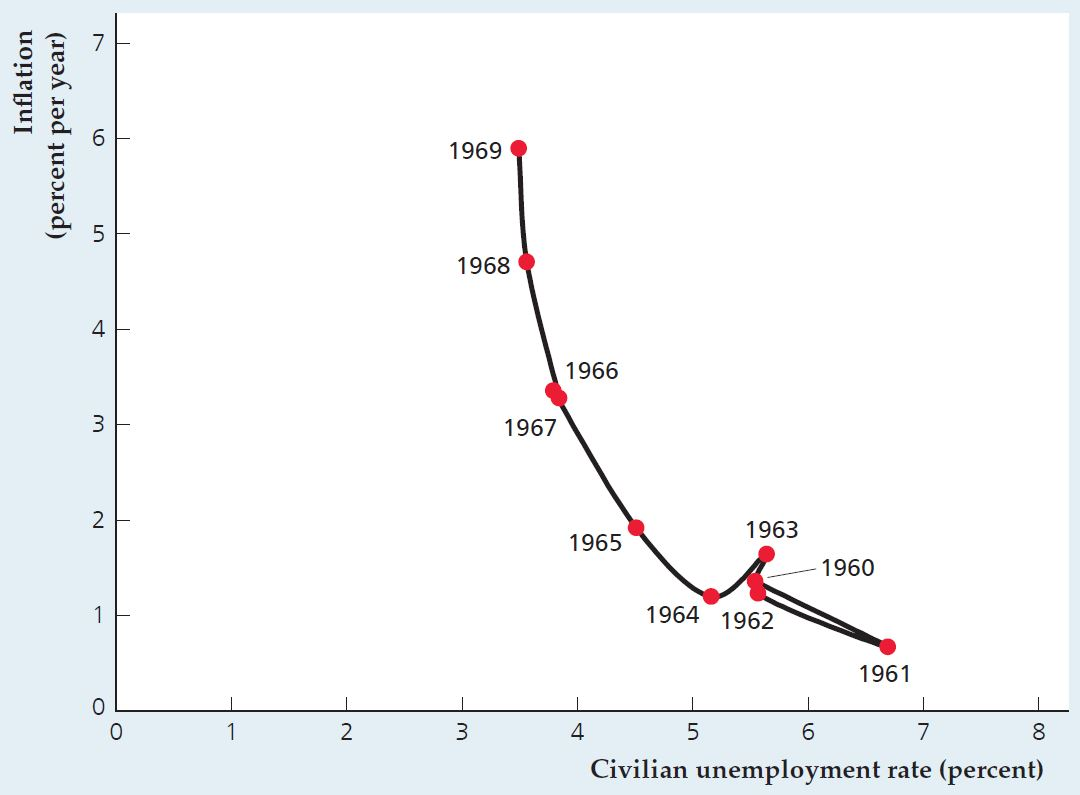
\includegraphics[width=0.5\textwidth]{./figures/aula13_fig6.JPG}
        \caption{A curva de Phillips e a economia dos EUA durante a década de 1960. Fonte: Abel et al. (2017).}
        \label{fig5}
    \end{figure}
\end{frame}

\begin{frame}{Introdução}
    \begin{itemize}
        \item Na década de 1970, no entanto, essa relação entre desemprego e inflação quebrou.
    \end{itemize}
    \begin{figure}
        \centering
        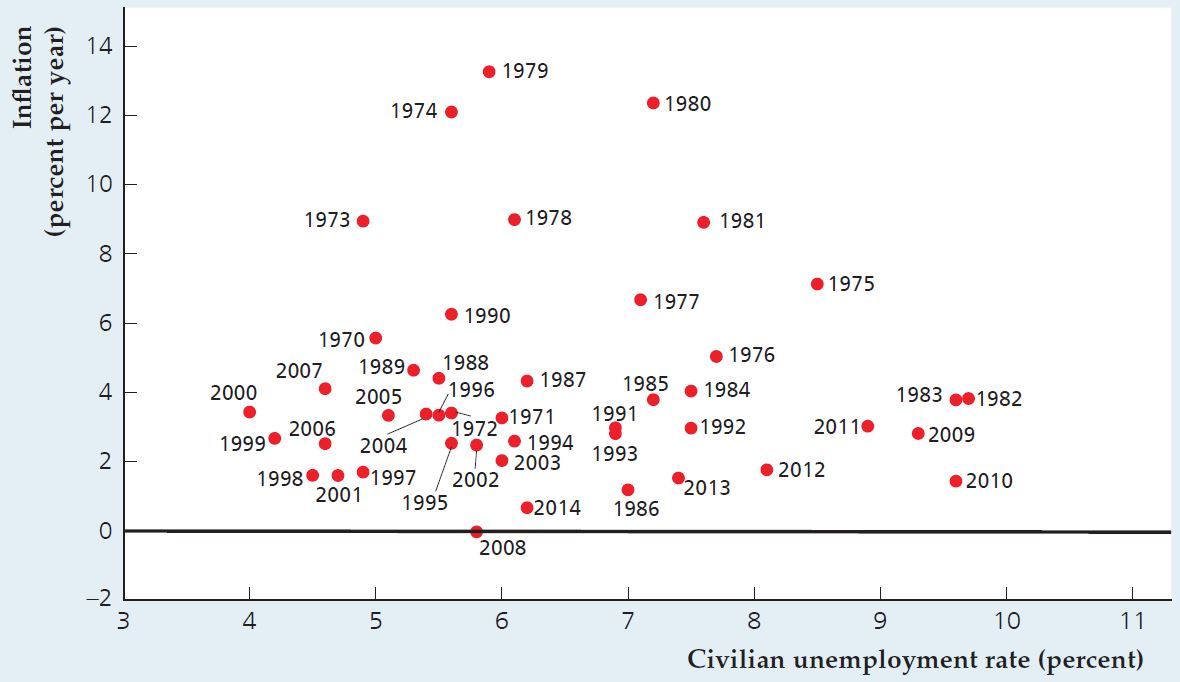
\includegraphics[width=0.7\textwidth]{./figures/aula13_fig7.JPG}
        \caption{Inflação e desemprego nos EUA, 1970-2014. Fonte: Abel et al. (2017).}
        \label{fig6}
    \end{figure}
\end{frame}

\begin{frame}{Introdução}
    \begin{itemize}
        \item Nos EUA, assim como na maioria dos países da OCDE, havia inflação alta \textcolor{blue}{e} desemprego alto (\textcolor{blue}{estagflação}), o que contradizia a curva de Phillips original.
        \bigskip
        \item Os resultados empíricos originalmente obtidos por Phillips e outros autores que estenderam seu trabalho, junto com a experiência inesperada das economias desenvolvidas após a década de 1970 sugerem, ao menos, três questões importantes:
        \bigskip
        \begin{enumerate}
            \item Por que a relação entre inflação e desemprego prevista originalmente na curva de Phillips foi frequentemente observada historicamente, como nos casos do UK antes de 1958 e dos EUA na década de 1960?
            \bigskip
            \item Por que essa relação entre desemprego e inflação quebrou após 1970?
            \bigskip
            \item A curva de Phillips, de fato, nos fornece um menu de opções com o qual os formuladores de política macroeconômica podem escolher?
        \end{enumerate}
    \end{itemize}
\end{frame}

\begin{frame}{Introdução}
    \begin{itemize}
        \item A teoria econômica nos fornece respostas razoáveis a todas estas questões.
        \bigskip
        \item Em particular, explica o colapso da curva de Phillips após 1970.
        \bigskip
        \item Surpreendentemente, a análise econômica fundamental da curva de Phillips - que previa que essa relação entre desemprego e inflação não era estável - foi feita durante a década de 1960, \textcolor{blue}{antes} mesmo que a curva de Phillips ``quebrasse''.
        \bigskip
        \item Temos, portanto, ao menos um exemplo de teoria econômica prevendo um desenvolvimento importante na economia que formuladores de política e o público não anteciparam.
        \bigskip
        \item Diante dos acontecimentos da década de 1970, uma relação entre inflação e desemprego ressurgiu, mas sob a forma de uma relação entre a taxa de desemprego e a \textcolor{blue}{variação} da taxa de inflação.
    \end{itemize}
\end{frame}

\section{Inflação, inflação esperada e desemprego}
\begin{frame}{Inflação, inflação esperada e desemprego}
    \begin{itemize}
        \item Nas aulas anteriores derivamos a seguinte equação de determinação de salários:
        \begin{equation}
            W = P^e F(u,z).
            \label{eq1}
        \end{equation}
        \bigskip
        \item O salário nominal, $W$, estabelecido pelos fixadores de salários, depende do nível esperado de preços, $P^e$, da taxa de desemprego, $u$, e de uma variável, $z$, que captura todos os outros fatores que afetam a determinação de salários, desde seguro-desemprego até a forma de negociação coletiva.
        \bigskip
        \item Vimos, também, a seguinte equação de fixação de preços:
        \begin{equation}
            P = (1 + m)W.
            \label{eq2}
        \end{equation}
        \bigskip
        \item O preço, $P$, estipulado pelas empresas (equivalentemente, o nível de preços) é igual ao salário nominal, $W$, vezes 1 mais o markup, $m$.
    \end{itemize}
\end{frame}

\begin{frame}{Inflação, inflação esperada e desemprego}
    \begin{itemize}
        \item Usamos, então, essas duas relações com a hipótese adicional de que o nível de preços observado era igual ao nível esperado de preços:
        \[
        P = P^e.
        \]
        \bigskip
        \item Sob essa hipótese, derivamos a taxa natural de desemprego e, via função de produção, o produto natural associado.
        \bigskip
        \item Esses dois conceitos representam o nível de equilíbrio para o qual o sistema econômico tende a convergir no médio prazo.
        \bigskip
        \item Nosso objetivo, agora, é explorar o que acontece quando não impomos a hipótese adicional de que $P = P^e$.
    \end{itemize}
\end{frame}

\begin{frame}{Inflação, inflação esperada e desemprego}
    \begin{itemize}
        \item Das equações (\ref{eq1}) e (\ref{eq2}), obtemos a seguinte expressão:
        \begin{equation}
            P = P^e (1 + m) F(u,z).
            \label{eq3}
        \end{equation}
        \bigskip
        \item Portanto, um aumento no nível esperado de preços leva a um aumento dos salários nominais (via fixação de salários) que, por sua vez, leva as empresas a elevarem seus preços (via fixação de preços), provocando uma elevação no nível de preços.
        \bigskip
        \item Um aumento da taxa de desemprego leva a uma redução dos salários nominais, o que, por sua vez, acarreta preços mais baixos e uma diminuição do nível de preços.
    \end{itemize}
\end{frame}

\begin{frame}{Inflação, inflação esperada e desemprego}
    \begin{itemize}
        \item Podemos adotar uma forma funcional linear para a função $F(u,z)$ da seguinte forma:
        \[
        F(u,z) = 1 - \alpha u + z.
        \]
        \bigskip
        \item O parâmetro $\alpha$ representa a força do efeito do desemprego sobre o salário.
        \bigskip
        \item Utilizando essa forma funcional na equação (\ref{eq3}), temos:
        \begin{equation}
            P = P^e (1 + m) (1-\alpha u + z).
            \label{eq4}
        \end{equation}
    \end{itemize}
\end{frame}

\begin{frame}{Inflação, inflação esperada e desemprego}
    \begin{itemize}
        \item A equação (\ref{eq4}) nos dá uma relação entre o nível de preços, o nível de preços esperado e a taxa de desemprego.
        \bigskip
        \item Nosso próximo passo é derivar uma relação entre inflação, inflação esperada e taxa de desemprego.
        \bigskip
        \item Incluindo índices temporais à equação (\ref{eq4}), temos:
        \[
        P_t = P^e_t (1 + m) (1-\alpha u_t + z).
        \]
        \bigskip
        \item Sabendo que a taxa de inflação, $\pi_t$, é dada por $(P_t - P_{t-1})/P_{t-1}$, manipulando a expressão anterior, podemos obter:
        \[
        1 + \pi_t = (1 + \pi_t^e)(1 + m)(1-\alpha u_t + z).
        \]
    \end{itemize}
\end{frame}

\begin{frame}{Inflação, inflação esperada e desemprego}
    \begin{itemize}
        \item Rearranjando os termos:
        \[
        \frac{(1 + \pi_t)}{(1 + \pi_t^e)(1 + m)} = (1-\alpha u_t + z).
        \]
        \bigskip
        \item Os seguintes resultados, obtidos via expansão de Taylor (para pequenas variações de $x$ e $y$), nos serão úteis:
        \begin{eqnarray*}
            (1 + x)(1 + y) &\approx& 1 + x + y, \\
            \frac{1 + x}{1 + y} &\approx& 1 + x - y.
        \end{eqnarray*}
        \bigskip
        \item Utilizando os resultados do item anterior, temos:
        \begin{equation*}
            1 + \pi_t - \pi_t^e - m = 1 - \alpha u_t + z.
        \end{equation*}
    \end{itemize}
\end{frame}

\begin{frame}{Inflação, inflação esperada e desemprego}
    \begin{itemize}
        \item Portanto, temos que:
        \begin{equation}
            \pi_t = \pi_t^e + (m + z) - \alpha u_t.
            \label{eq5}
        \end{equation}
        \bigskip
        \item Desconsiderando os subíndices temporais, a equação (\ref{eq4}) pode ser reescrita como:
        \begin{equation}
            \pi = \pi^e + (m + z) - \alpha u.
            \label{eq6}
        \end{equation}
    \end{itemize}
\end{frame}

\begin{frame}{Inflação, inflação esperada e desemprego}
    \begin{equation*}
        \pi = \pi^e + (m + z) - \alpha u.
    \end{equation*}
    \bigskip
    \begin{itemize}
        \item \textcolor{blue}{Um aumento da inflação esperada, $\pi^e$, leva a um aumento da inflação efetiva, $\pi$.}
        \bigskip
        \item Um aumento do nível esperado de preços leva a um aumento de igual magnitude do nível de preços efetivo. Se os fixadores de salários esperam um nível de preços mais elevado, fixam um salário nominal mais elevado, o que aumenta o nível de preços.
        \bigskip
        \item Dado o nível de preços do período anterior, um nível de preços e de preços esperados mais altos neste período implicam, respectivamente, uma taxa de inflação e inflação esperada mais altas.
        \bigskip
        \item Portanto, um aumento da inflação esperada leva a um aumento da inflação efetiva.
    \end{itemize}
\end{frame}

\begin{frame}{Inflação, inflação esperada e desemprego}
    \begin{equation*}
        \pi = \pi^e + (m + z) - \alpha u.
    \end{equation*}
    \bigskip
    \begin{itemize}
        \item \textcolor{blue}{Dada a inflação esperada, $\pi^e$, um aumento do markup, $m$, ou da variável abrangente $z$ leva a um aumento da inflação, $\pi$.}
        \bigskip
        \item Dado o nível esperado de preços, $P^e$, um aumento de $m$ ou de $z$ leva a um aumento do nível de preços, $P$.
        \bigskip
        \item Portanto, usando o mesmo argumento anterior, temos: dada a inflação esperada, um aumento de $m$ ou de $z$ leva a um aumento da inflação efetiva.
    \end{itemize}
\end{frame}

\begin{frame}{Inflação, inflação esperada e desemprego}
    \begin{equation*}
        \pi = \pi^e + (m + z) - \alpha u.
    \end{equation*}
    \bigskip
    \begin{itemize}
        \item \textcolor{blue}{Dada a inflação esperada, $\pi^e$, uma diminuição da taxa de desemprego, $u$, leva a um aumento da inflação, $\pi$.}
        \bigskip
        \item Dado o nível esperado de preços, $P^e$, uma redução da taxa de desemprego leva a um salário nominal mais alto o que, por sua vez, eleva o nível de preços efetivo.
        \bigskip
        \item Portanto, usando o mesmo argumento anterior, temos: dada a taxa de inflação esperada, $\pi^e$, um aumento da taxa de desemprego, $u$, leva a uma diminuição da inflação efetiva, $\pi$.
    \end{itemize}
\end{frame}

\section{Evolução da curva de Phillips}
\subsection{Phillips, Solow e Samuelson}
\begin{frame}{A curva de Phillips original}
    \begin{itemize}
        \item Suponhamos que a inflação varie de um ano para o outro em torno de algum valor estacionário $\bar{\pi}$.
        \bigskip
        \item Suponhamos, também, que a taxa de inflação não seja persistente, de modo que a inflação deste ano não sirva de parâmetro para a do próximo ano.
        \bigskip
        \item Estas hipóteses são satisfatórias para o comportamento da inflação no período analisado por Phillips, Samuelson e Solow.
        \bigskip
        \item Neste caso, faz sentido que os fixadores de salários assumam que, qualquer que seja a inflação do ano anterior, a inflação do ano presente será igual a $\bar{\pi}$, ou seja:
        \[
        \pi^e_t = \bar{\pi}.
        \]
    \end{itemize}
\end{frame}

\begin{frame}{A curva de Phillips original}
    \begin{itemize}
        \item Portanto, temos que:
        \begin{equation}
        \pi_t = \bar{\pi} + (m + z) - \alpha u_t.
        \label{eq7}
        \end{equation}
        \bigskip
        \item Neste caso, observaremos uma relação negativa entre taxa de desemprego e taxa de inflação.
        \bigskip
        \item Esta é, precisamente, a relação negativa entre desemprego e inflação que Phillips encontrou para o UK, e Solow e Samuelson para os EUA.
        \bigskip
        \item Quando o desemprego era elevado, a inflação era baixa - ou até negativa.
        \bigskip
        \item Quando o desemprego era baixo, a inflação era alta.
    \end{itemize}
\end{frame}

\subsection{Trade-off aparente desemprego $\times$ inflação}
\begin{frame}{Trade-off aparente desemprego $\times$ inflação}
    \begin{itemize}
        \item Os resultados empíricos obtidos por Phillips, Samuelson e Solow sugeriam que os formuladores de política econômica estavam diante de um trade-off entre inflação e desemprego.
        \bigskip
        \item Se estivessem dispostos a aceitar mais inflação, poderiam atingir um desemprego menor.
        \bigskip
        \item Este parecia ser um trade-off atraente e, a partir dos anos 1960, a política macroeconômica norte-americana visou reduzir continuamente o desemprego. 
    \end{itemize}
\end{frame}

\begin{frame}{Trade-off aparente desemprego $\times$ inflação}
    \begin{figure}
        \centering
        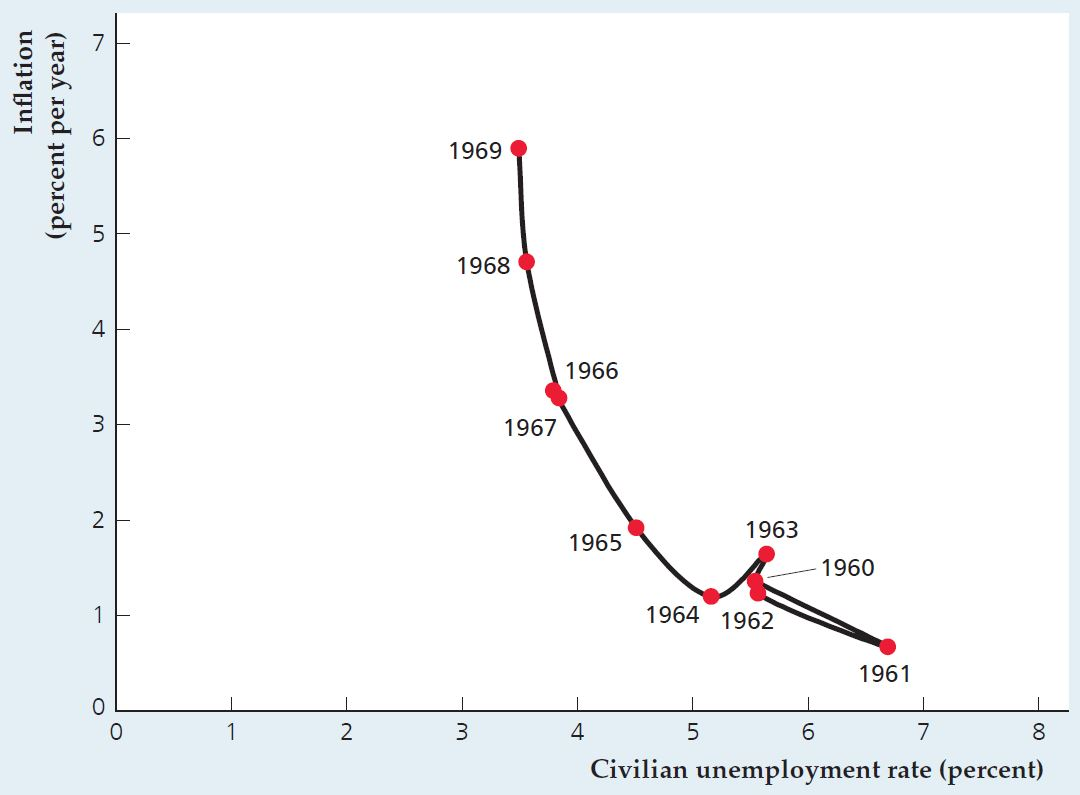
\includegraphics[width=0.6\textwidth]{./figures/aula13_fig6.JPG}
        \caption{A curva de Phillips e a economia dos EUA durante a década de 1960. Fonte: Abel et al. (2017).}
        \label{fig7}
    \end{figure}
\end{frame}

\begin{frame}{Trade-off aparente desemprego $\times$ inflação}
    \begin{itemize}
        \item Observe, na Figura \ref{fig7}, como a relação entre desemprego e inflação - alinhada à equação (\ref{eq7}) - se manteve durante a longa expansão econômica de quase toda a década de 1960.
        \bigskip
        \item De 1961 a 1969, a taxa de desemprego baixou continuamente, de 6,8\% para 3,4\%.
        \bigskip
        \item A taxa de inflação, por sua vez, subiu de aproximadamente 1\% para aproximadamente 6\%.
        \bigskip
        \item De modo informal, a economia dos EUA deslocou-se para cima ao longo da curva de Phillips original.
        \bigskip
        \item Realmente parecia que, se os formuladores de política econômica estivessem dispostos a aceitar uma inflação mais elevada, poderiam atingir um desemprego mais baixo.
    \end{itemize}
\end{frame}

\begin{frame}{Trade-off aparente desemprego $\times$ inflação}
    \begin{itemize}
        \item Entretanto, a relação entre taxa de desemprego e taxa de inflação parece ter quebrado na década de 1970.
    \end{itemize}
    \begin{figure}
        \centering
        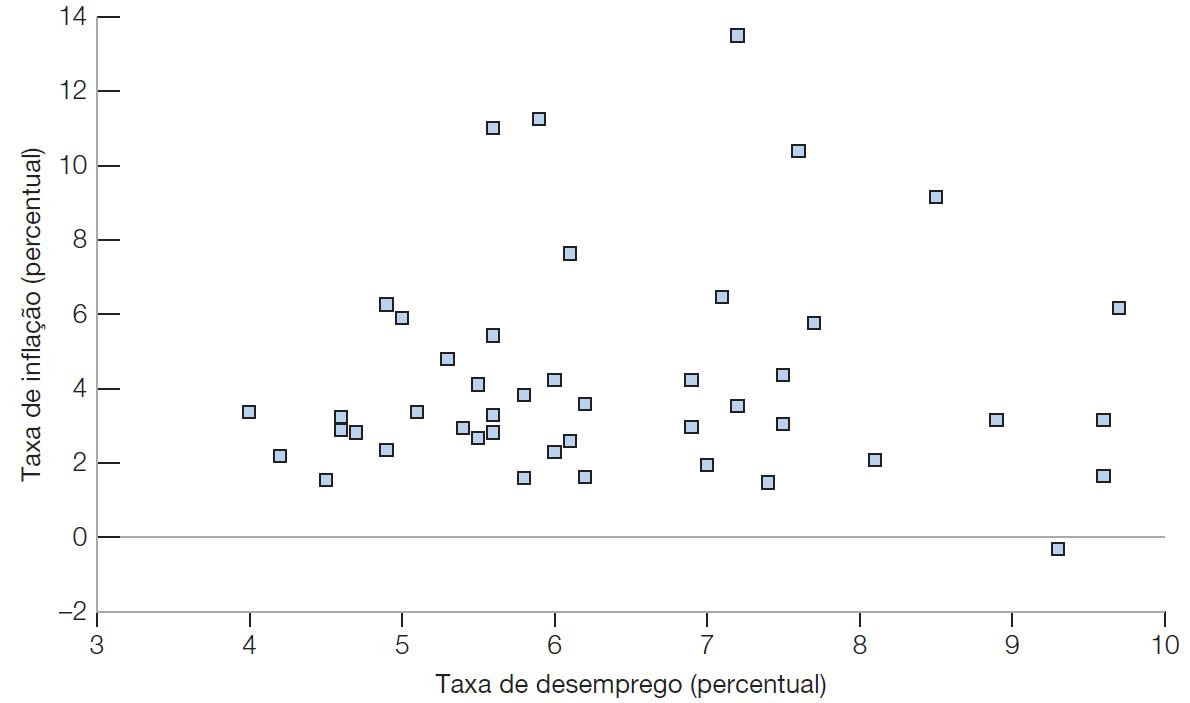
\includegraphics[width=0.6\textwidth]{./figures/aula13_fig8.JPG}
        \caption{Inflação $\times$ desemprego, EUA (1970-2014). Fonte: Blanchard (2017).}
        \label{fig8}
    \end{figure}
\end{frame}

\begin{frame}{Trade-off aparente desemprego $\times$ inflação}
    \begin{itemize}
        \item A Figura \ref{fig8} evidencia que não existe mais qualquer relação visível entre a taxa de desemprego e a taxa de inflação.
        \bigskip
        \item Por que a curva de Phillips original desapareceu?
        \bigskip
        \item Porque os fixadores de salários mudaram o modo como formavam suas expectativas em relação à inflação.
        \bigskip
        \item Essa mudança veio de uma alteração no comportamento da inflação.
        \bigskip
        \item A inflação tornou-se mais persistente.
    \end{itemize}
\end{frame}

\begin{frame}{Trade-off aparente desemprego $\times$ inflação}
    \begin{itemize}
        \item O aumento na persistência da inflação significa um aumento na probabilidade de a inflação alta de um ano ser seguida por uma inflação alta no ano seguinte.
        \bigskip
        \item Assim, os agentes econômicos ao formarem suas expectativas incorporaram essa informação acerca da persistência da inflação.
        \bigskip
        \item Essa mudança na formação de expectativas acabou por modificar a natureza da relação entre desemprego e inflação.
    \end{itemize}
\end{frame}

\begin{frame}{Trade-off aparente desemprego $\times$ inflação}
    \begin{itemize}
        \item Suponha, agora, que as expectativas de inflação sejam formadas de acordo com a seguinte equação:
        \begin{equation}
            \pi_t^e = (1 - \theta) \bar{\pi} + \theta \pi_{t-1}.
            \label{eq8}
        \end{equation}
        \bigskip
        \item Portanto, quanto maior $\theta$, maior o peso que a inflação do período anterior terá sobre as expectativas de firmas e trabalhadores acerca do nível de preços e, portanto, maior a taxa de inflação esperada.
    \end{itemize}
\end{frame}

\begin{frame}{Trade-off aparente desemprego $\times$ inflação}
    \begin{itemize}
        \item Podemos pensar no que aconteceu na década de 1970 como um aumento do valor de $\theta$ ao longo do tempo:
        \bigskip
        \begin{enumerate}
            \item Enquanto a persistência da inflação era baixa, firmas e trabalhadores ignoravam a inflação do período anterior e, portanto, admitiam um valor constante para a inflação. Ou seja, $\theta \approx 0$ - $\pi_t^e \approx \bar{\pi}$ e curva de Phillips dada pela equação (\ref{eq7}).
            \bigskip
            \item À medida que a inflação se tornava mais persistente, trabalhadores e firmas começaram a mudar o modo de formar expectativas. Se a inflação foi alta no período anterior, provavelmente seria alta no período seguinte. Ou seja, $\theta$ aumentaria. As evidências sugerem que, em meados da década de 1970, as pessoas formavam suas expectativas esperando que a taxa de inflação do ano atual seria igual à do ano anterior - $\theta = 1$.
        \end{enumerate}
    \end{itemize}
\end{frame}

\begin{frame}{Trade-off aparente desemprego $\times$ inflação}
    \begin{itemize}
        \item Para examinar as implicações de valores distintos de $\theta$ sobre o trade-off inflação $\times$ desemprego, temos:
        \begin{equation}
            \pi_t = (1 - \theta) \bar{\pi} + \theta \pi_{t-1} + (m + z) - \alpha u_t.
            \label{eq9}
        \end{equation}
        \bigskip
        \begin{enumerate}
            \item Se $\theta = 0$, obtemos a curva de Phillips original com uma relação entre taxa de desemprego e taxa de inflação.
            \bigskip
            \item Se $0 < \theta < 1$, a taxa de inflação depende não só da taxa de desemprego mas, também, da taxa de inflação do ano anterior:
            \[
            \pi_t = [(1 - \theta) \bar{\pi} + (m + z)] + \theta \pi_{t-1}  - \alpha u_t.
            \]
            \bigskip
            \item Se $\theta = 1$ ($\pi_t^e = \pi_{t-1}$ - expectativas adaptativas), temos:
            \begin{equation}
            \pi_t - \pi_{t-1} = (m + z) - \alpha u_t.
            \label{eq10}
            \end{equation}
        \end{enumerate}
    \end{itemize}
\end{frame}

\begin{frame}{Trade-off aparente desemprego $\times$ inflação}
    \begin{itemize}
        \item Portanto, quando $\theta = 1$, a taxa de desemprego afeta não a \textcolor{red}{taxa de inflação}, mas a \textcolor{blue}{variação da taxa de inflação}:
        \[
        \Delta \pi_t = (m + z) - \alpha u_t.
        \]
        \bigskip
        \item O desemprego elevado leva a uma inflação decrescente.
        \bigskip
        \item O desemprego baixo leva a uma inflação crescente.
    \end{itemize}
\end{frame}

\begin{frame}{Trade-off aparente desemprego $\times$ inflação}
    \begin{itemize}
        \item Essa discussão é fundamental para o que aconteceu na década de 1970.
        \bigskip
        \item Quando $\theta$ aumentou de zero para 1, a relação simples entre taxa de desemprego e taxa de inflação desapareceu.
        \bigskip
        \item Esse desaparecimento foi o que vimos nas Figuras \ref{fig6} e \ref{fig8}.
        \bigskip
        \item Mas uma nova relação surgiu - entre taxa de desemprego e variação da taxa de inflação.
    \end{itemize}
\end{frame}

\begin{frame}{Trade-off aparente desemprego $\times$ inflação}
    \begin{itemize}
        \item Essa relação entre taxa de desemprego e variação da taxa de inflação é representada na Figura \ref{fig9}
    \end{itemize}
    \begin{figure}
        \centering
        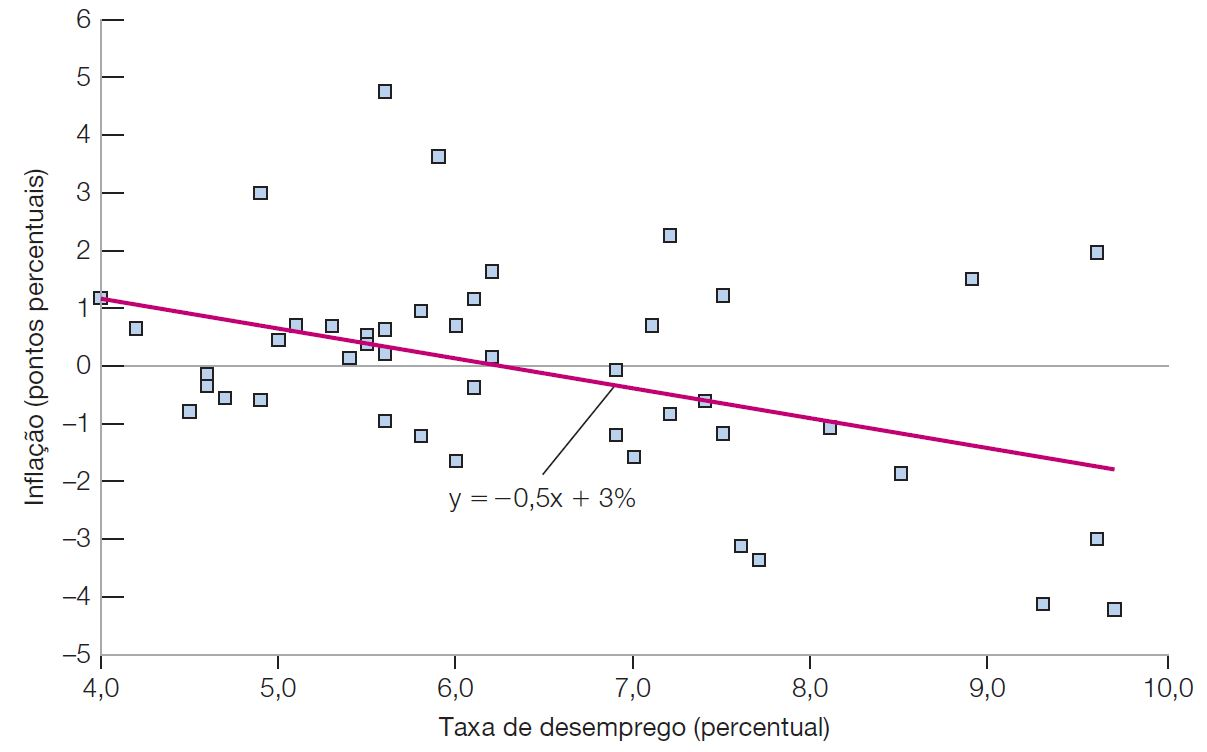
\includegraphics[width = 0.6\textwidth]{./figures/aula13_fig9.JPG}
        \caption{Variação da inflação $\times$ desemprego, EUA (1970 - 2014). Fonte: Blanchard (2017).}
        \label{fig9}
    \end{figure}
\end{frame}

\begin{frame}{Trade-off aparente desemprego $\times$ inflação}
    \begin{itemize}
        \item A reta de regressão que melhor se ajusta para o período 1970-2014 na economia norte-americana, segundo Blanchard, é dada por:
        \[
        \Delta \pi_t = 3,0\% - 0,5 u_t.
        \]
        \bigskip
        \item Para um desemprego baixo, a variação da inflação é positiva.
        \bigskip
        \item Para um desemprego alto, a variação da inflação é negativa.
        \bigskip
        \item Para diferenciá-la da curva de Phillips original (\ref{eq7}), a equação (\ref{eq10}) ou sua contraparte empírica é chamada de \textcolor{blue}{curva de Phillips modificada}, \textcolor{blue}{curva de Phillips aumentada pelas expectativas} ou, ainda, \textcolor{blue}{curva de Phillips aceleracionista}.
    \end{itemize}
\end{frame}

\section{Bibliografia}
\begin{frame}{\emoji{books} Bibliografia}
    \begin{itemize}                
        \item BLANCHARD, O. Macroeconomia. 7.ed. São Paulo: Pearson Education do Brasil, 2017\medskip                
        \item CARLIN, W.; SOSKICE, D. Macroeconomics: Institutions, instability, and the financial system. Oxford, UK: Oxford University Press, 2015\medskip        
        \item DORNBUSCH, R.; FISCHER, S.; STARTZ, R. Macroeconomia. 11.ed. Porto Alegre: AMGH, 2013. Disponível em: \href{https://app.minhabiblioteca.com.br/books/9788580551853}{app.minhabiblioteca.com.br/books/9788580551853}\medskip
        \item FROYEN, R. Macroeconomia: teorias e aplicações. 2.ed. São Paulo: Saraiva, 2013. Disponível em: \href{https://app.minhabiblioteca.com.br/books/9788502175235}{app.minhabiblioteca.com.br/books/9788502175235}        
    \end{itemize}
\end{frame}
\end{document}